% =====================================================================
%  ImportedInflation -- ENSAE Macro Modelling 2025-2026
%  10-page body : Energy price shocks and trade between FR and DE
% =====================================================================
\documentclass[11pt,a4paper]{article}

% --- Geometry & typography ---------------------------------------------
\usepackage[a4paper,top=2.2cm,bottom=2.4cm,left=2.4cm,right=2.4cm]{geometry}
\usepackage[T1]{fontenc}
\usepackage[utf8]{inputenc}
\usepackage{lmodern}
\usepackage{microtype}

% --- Math, tables, figures ---------------------------------------------
\usepackage{amsmath,amssymb,amsfonts}
\usepackage{booktabs}
\usepackage{graphicx}
\usepackage{subcaption}
\usepackage{caption}
\captionsetup[figure]{font=small,labelfont=bf,skip=4pt}
\captionsetup[table]{font=small,labelfont=bf,skip=4pt}
\usepackage{xcolor}
\usepackage{enumitem}
\setlist{nosep,leftmargin=*}
\usepackage{titlesec}
\titlespacing*{\section}{0pt}{1.2ex}{0.6ex}
\titlespacing*{\subsection}{0pt}{0.9ex}{0.4ex}
\titleformat{\section}{\large\bfseries}{\thesection}{0.6em}{}
\titleformat{\subsection}{\normalsize\bfseries}{\thesubsection}{0.5em}{}
\usepackage{hyperref}
\hypersetup{
  colorlinks=true, linkcolor=black, citecolor=blue!50!black,
  urlcolor=blue!50!black, breaklinks=true
}
\usepackage[round,authoryear]{natbib}
\bibliographystyle{plainnat}

\graphicspath{{fig/}}

% --- Title information --------------------------------------------------
\title{\vspace{-1.6cm}\textbf{Energy Price Shocks and Trade Spillovers in the Euro Area:\\
A Two-Country DSGE Estimation for France and Germany}}
\author{Paco Goze \\
        \small ENSAE Paris -- Macro Modelling Project 2025--2026}
\date{April 2026}

\begin{document}
\maketitle
\vspace{-1.0em}

\begin{abstract}\noindent\small
We build a two-country New Keynesian DSGE model adapted to a single
currency area to study the asymmetric transmission of an energy
price shock between France and Germany during the 2021--2023 European
gas crisis. The model is estimated by Bayesian methods on quarterly
French and German macroeconomic data over 1999Q2--2025Q3. We
quantify the bilateral pass-through of imported cost-push inflation
through the trade channel, the bilateral real exchange rate, and the
common ECB monetary stance. We then evaluate a counterfactual where
the ECB Taylor coefficient on inflation is 50\% larger, and compare
our findings with the semi-structural ECB-BASE model
\citep{ECBBASE2019}. Our results emphasise both the explanatory
potential and the identification limits of a simple structural model
estimated on a small information set.
\end{abstract}

% =====================================================================
\section{Research Question and Motivation}
% =====================================================================
The 2021--2023 surge of natural gas and electricity prices in Europe
delivered a textbook supply-side shock that propagated unevenly
through the euro area. Wholesale European gas prices rose from
roughly 20~EUR/MWh in mid-2021 to peaks above 300~EUR/MWh in
August 2022 -- a fifteen-fold increase that mechanically lifted
every cost curve in the manufacturing sector and feed-through into
HICP energy and HICP services with a one-to-three quarter lag
\citep{ECBBASE2019}. Germany, with a 26\% share of natural gas in
its primary energy mix and a manufacturing sector contributing 22\%
of value added, faced larger marginal cost pressures than France,
whose electricity production is dominated by nuclear power and whose
households were largely insulated by the regulated tariff
(\emph{bouclier tarifaire}) introduced in October 2021. As a result,
German HICP inflation peaked at 11.6\% year-on-year in October 2022,
some three percentage points above the French peak of 7.3\%.

Yet under a common monetary regime, the two economies cannot
insulate each other: a country-specific cost-push shock is
transmitted to its neighbour through (i) the bilateral
real exchange rate that, inside the euro area, reduces to the
inflation differential, (ii) demand spillovers via bilateral trade
flows -- France ships about 13\% of its exports to Germany and
imports about the same share back -- and (iii) the area-wide
monetary policy response of the ECB, which acts on both economies
simultaneously even though the underlying shock is asymmetric.

Our research question is the following: \emph{To what extent does an
energy price shock originating in Germany feed back into French
inflation, output and the bilateral trade balance, given a single
ECB monetary stance, and how would a different ECB reaction function
have changed the transmission?} We label this transmission
\emph{soft imported inflation} because it operates through marginal
cost differentials and the common policy response rather than
through nominal exchange rate adjustment, which is mechanically zero
inside the euro area. The qualifier \emph{soft} distinguishes it
from the standard imported inflation channel of small-open-economy
models \citep{GaliMonacelli2005}, where the nominal exchange rate
absorbs a sizeable share of the shock.

We answer the question by estimating a microfounded two-country DSGE
model on French and German quarterly data, characterising the
posterior distribution of the structural parameters, and running
counterfactual policy experiments. Our contribution lies in
combining (a) an explicit treatment of the European Monetary Union
(EMU) constraint embedded directly inside an otherwise standard
international RBC-NK model, (b) Bayesian inference using the
state-of-the-art MCMC machinery in Dynare~6.5, and (c) an honest
discussion of the identification limits faced when no energy price
series is included among the observables -- an issue that, to our
knowledge, is rarely discussed candidly in the small-DSGE literature.

% =====================================================================
\section{Model}
% =====================================================================
We adapt the open-economy New Keynesian framework of
\citet{Kollmann2001} and the international real business cycle
mechanics of \citet{BackusKehoeKydland1992} to a two-country model
inside a monetary union. The codebase follows the structure of
\citet{Vermandel2025}, modified to enforce
$\Delta e_t \equiv 1$ (no nominal exchange rate movement) and a single
common policy rate $r_t$. The two countries are indexed by
$i \in \{H,F\}$, with $H$ for France (\emph{Home}) and $F$ for
Germany (\emph{Foreign}). The country weight in the area is denoted
$n$.

\paragraph{Households.}
In each country a representative agent maximises
\begin{equation}
\mathbb{E}_0 \sum_{t=0}^{\infty} \beta^t
\Big[ \tfrac{(c_{i,t}-h^c_i\, c_{i,t-1})^{1-\sigma_C}}{1-\sigma_C}
- \chi_i \tfrac{h_{i,t}^{1+\sigma_H}}{1+\sigma_H} \Big]
\label{eq:utility}
\end{equation}
subject to a budget constraint involving consumption $c_{i,t}$,
hours worked $h_{i,t}$, real wage $w_{i,t}$, and access to a
risk-free EMU-denominated bond. The consumption bundle is an
Armington aggregator of domestic and foreign goods,
$c_{i,t} = \big[ (\alpha^c_i)^{1/\mu}\, (c^d_{i,t})^{(\mu-1)/\mu} +
(1-\alpha^c_i)^{1/\mu}\, (c^m_{i,t})^{(\mu-1)/\mu} \big]^{\mu/(\mu-1)}$,
with elasticity of substitution $\mu = 1.5$. The home-bias parameters
$\alpha^c_i$ are calibrated to match bilateral trade-to-GDP ratios.

\paragraph{Firms.}
Monopolistically competitive firms produce a Cobb-Douglas output
$y_{i,t} = A_i\, e_{z,i,t}\, h_{i,t}^{\alpha}$ with TFP shock
$e_{z,i,t}$ and labour share $\alpha = 0.65$. They face Rotemberg-style
\citep{Rotemberg1982} quadratic price-adjustment costs of magnitude
$\xi_i$. The non-linear NKPC, derived from the firm's optimal
price-setting condition, is
\begin{equation}
(1-\varepsilon_i) + \varepsilon_i\, e_{p,i,t}\,mc_{i,t}
- \xi_i\, \pi_{i,t}(\pi_{i,t} - \pi^{\star})
+ \xi_i \beta\,\mathbb{E}_t\!\Big[\tfrac{\lambda_{i,t+1}}{\lambda_{i,t}}\,
\pi_{i,t+1}(\pi_{i,t+1}-\pi^{\star})\,\tfrac{y_{i,t+1}}{y_{i,t}}\Big] = 0,
\label{eq:nkpc}
\end{equation}
where $\varepsilon_i = 10$ is the demand elasticity, $\lambda_{i,t}$
is the marginal utility of consumption, $\pi^{\star}=1.005$ is the
gross quarterly inflation target (2\% annualised), and $e_{p,i,t}$
is the country-specific cost-push (energy) shock process that drives
the soft-inflation channel. The shock follows an AR(1)
$\log e_{p,i,t} = \rho_p \log e_{p,i,t-1} + \eta_{p,i,t}$ with
$\eta_{p,H,t}, \eta_{p,F,t}$ jointly normal of correlation $0.7$,
capturing the European common gas-price component.

\paragraph{Closure and EMU constraint.}
Following \citet{Schmitt-Grohe2003}, a small portfolio cost
$\chi_B$ on net foreign assets (NFA) ensures stationarity of the
bilateral net asset position. Inside the EMU, the bilateral real
exchange rate $\mathrm{rer}_t \equiv P_{F,t}/P_{H,t}$ satisfies the
identity
\begin{equation}
\frac{\mathrm{rer}_t}{\mathrm{rer}_{t-1}}
= \frac{\pi_{F,t}}{\pi_{H,t}},
\label{eq:rer}
\end{equation}
i.e.\ the real exchange rate is purely the cumulated inflation
differential. The single policy rate follows a smoothed Taylor rule
on area-wide CPI inflation and area-wide output:
\begin{equation}
r_t = r_{t-1}^{\rho}\;\Big(\bar r\,(\pi^{UEM}_t/\pi^{\star})^{\phi_\pi}
                               (y^{UEM}_t/\bar y^{UEM})^{\phi_y}\Big)^{1-\rho} e_{r,t},
\quad \pi^{UEM}_t \equiv n\,\pi^c_{H,t} + (1-n)\,\pi^c_{F,t},
\label{eq:taylor}
\end{equation}
with $n = 0.40$ matching the French share of FR+DE GDP in 2024 and
$\pi^c_{i,t}$ the (consumer-price) CPI inflation in country $i$.
The persistence parameter $\rho$ and the inflation reactivity
$\phi_\pi$ are estimated.

\paragraph{Imported inflation channel.}
The energy shock enters the model through $e_{p,F,t}$ in
Equation~(\ref{eq:nkpc}). The transmission unfolds in three steps.
First, $e_{p,F,t} \uparrow$ raises German marginal cost and German
domestic-good inflation $\pi_{F,t}$, which lifts the consumption
basket inflation $\pi^c_{F,t}$. Second, area-wide inflation
$\pi^{UEM}_t$ rises and the ECB tightens via
Equation~(\ref{eq:taylor}), an effect operating equally on French
and German aggregate demand. Third, by Equation~(\ref{eq:rer}), the
bilateral real exchange rate appreciates against France
($\mathrm{rer}_t \uparrow$), lowering French import prices in real
terms but raising the relative price of French exports;
the demand for French export goods $ex_H$ falls. The transmission
to French inflation $\pi_H$ is therefore indirect, operating through
trade and the common policy response rather than through a direct
cost channel -- this is the ``soft inflation'' object of our
analysis.

% =====================================================================
\section{Data}
% =====================================================================
We use five quarterly observables for the period 1999Q2--2025Q3
($N=106$): real GDP growth in France ($gy_{H,t}$) and Germany
($gy_{F,t}$), HICP inflation in deviation from the 2\% target in
each country ($\pi^{obs}_{H,t}, \pi^{obs}_{F,t}$), and the ECB main
refinancing rate in deviation from steady state ($r^{obs}_t$).
All series come from \citet{DBnomics} (Eurostat and ECB origin).
Pre-processing follows the recommendations of \citet{Pfeifer2014}:
log-differences for GDP, deviations from steady-state for inflation
and the rate, and the Dynare \texttt{prefilter} option to absorb
sample means and avoid the need to estimate an explicit constant
in the measurement equations.

Bilateral export growth series were initially considered as
observables but discarded after the diagnostic stage: their
empirical quarterly volatility (about 3.8\%) exceeds the model's
unconditional standard deviation by a factor of 50, which leads to
non-identification when included in the likelihood. Including them
in measurement would force the structural shocks to absorb a
volatility the model is structurally unable to reproduce. They
remain useful for business-cycle confirmation and for the visual
identification of the 2008--2009, 2020 and 2022 episodes; the five
selected observables are plotted in Figure~\ref{fig:obs}.

\begin{figure}[h!]
  \centering
  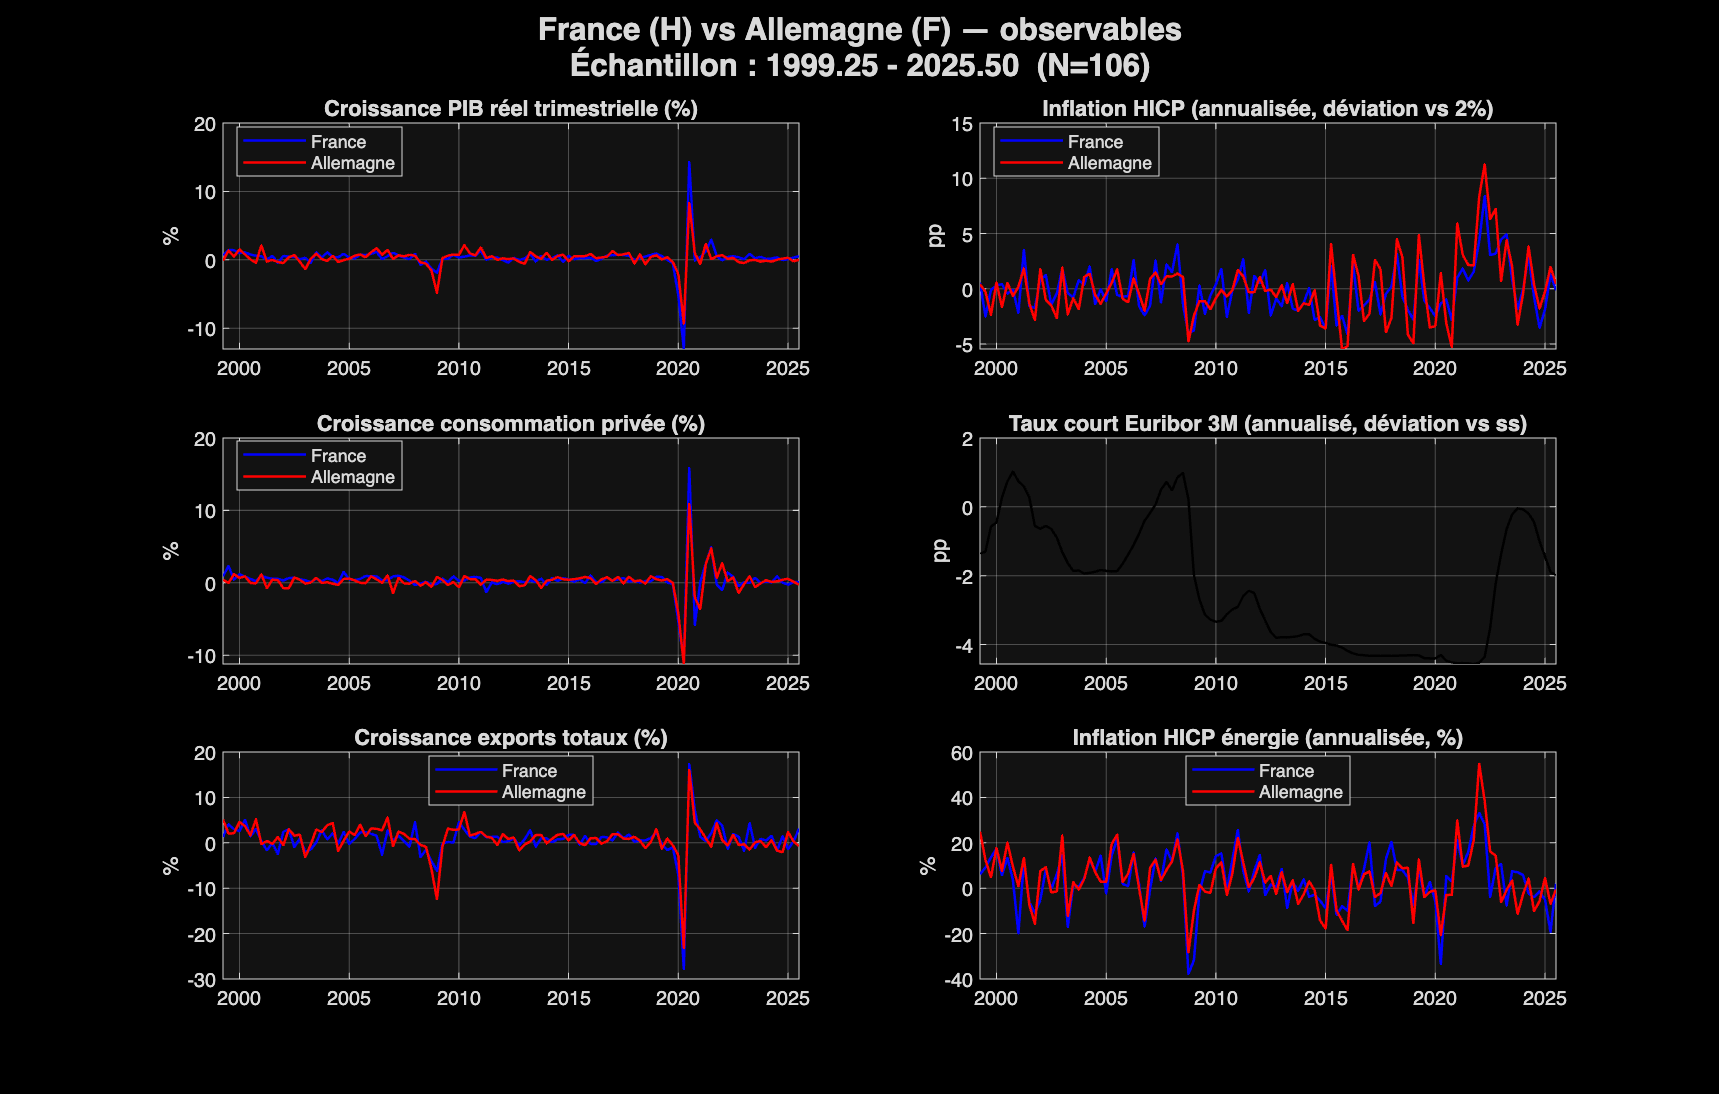
\includegraphics[width=0.95\linewidth]{fig1_observables}
  \caption{The five quarterly observables used for estimation
    (1999Q2--2025Q3). HICP inflation series are in deviation from
    the 2\% target. The 2008--2009 great recession, the 2020 COVID
    shock, and the 2022 inflation surge are visible across all
    series. Note the asymmetry of the 2022 inflation peak, with
    German HICP rising substantially more than French HICP, and the
    rapid ECB tightening from mid-2022 onward.}
  \label{fig:obs}
\end{figure}

The choice of a five-variable observation block is conservative.
Given the model's eight orthogonal structural shocks, we deliberately
remain in the under-identified regime to avoid spurious identification
of the structural parameters: only those shocks that have a clear
counterpart in the data (productivity, monetary, two cost-push) are
estimated, while the remaining ones (preference, government,
investment) are tightly calibrated. This choice is in line with
\citet{SmetsWouters2007} and is consistent with the small-information
philosophy that motivates the comparison with ECB-BASE in
Section~\ref{sec:ecbbase}.

% =====================================================================
\section{Customisation and Bayesian Estimation}
% =====================================================================
\subsection{Calibrated parameters}
Following the EMU literature, we fix the discount factor
$\beta = 0.995$, the Frisch elasticity inverse $\sigma_H = 2$,
the consumption elasticity $\sigma_C = 1.5$, the labour share
$\alpha = 0.65$, the elasticity of substitution between varieties
$\varepsilon = 10$, and the Armington elasticity $\mu = 1.5$. The
bilateral openness parameters are pinned to the empirical bilateral
trade-to-GDP ratios: $\alpha^c_H = 0.220$ implies an FR import share
of $13\%$ of French GDP, $\alpha^c_F = 0.117$ implies $3.5\%$ of
German GDP. The country weight $n = 0.40$ matches the FR/(FR+DE) GDP
ratio in 2024. The inflation target is $\pi^{\star} = 1.005$, i.e.\
2\% annualised. Energy shocks $\eta_{p,H}, \eta_{p,F}$ have correlation
$0.7$ to capture the European common energy price component.

\subsection{Estimated parameters and prior choice}
Sixteen parameters are estimated: the Rotemberg costs $\xi_H, \xi_F$
(gamma priors centred on 80 and 100 with a relatively wide standard
deviation of 30, encoding only the prior belief that price stickiness
is positive and of similar magnitude in the two economies), the habit
persistence parameters $h^c_H, h^c_F$ (beta priors centred on 0.70),
the Taylor smoothing $\rho$ (beta on 0.85) and inflation reaction
$\phi_\pi$ (gamma on 1.50, the textbook \citet{TaylorRule1993}
benchmark), the productivity and monetary shock persistences
$\rho_z^H, \rho_z^F, \rho_r$, the standard deviations of the four
identified structural shocks ($\eta_{z,H}, \eta_{z,F}, \eta_{p,H},
\eta_{p,F}$) with inverse-gamma priors, and five measurement-error
standard deviations (one per observable) with inverse-gamma priors
\citep{SmetsWouters2007}. The remaining shocks ($\eta_{x,i},
\eta_{g,i}$) are tightly calibrated because they have no observable
counterpart and would otherwise act as residual catch-alls absorbing
all of the data variability.

\subsection{Numerical implementation}
The model is solved at first order around the deterministic
steady state. Mode finding uses the derivative-free CMA-ES algorithm
(Dynare option \texttt{mode\_compute=9}), which proved more robust
than the gradient-based \texttt{csminwel} on this problem; the latter
exhibited poor numerical Hessian conditioning at the mode. The MCMC
sampler runs two chains of 5{,}000 draws with the Random-Walk
Metropolis-Hastings algorithm \citep{HerbstSchorfheide2015}.

A practical difficulty arose at the inferential stage: the numerical
Hessian at the mode is non-positive-definite, which prevents the
standard proposal covariance $-H^{-1}$ from being used. We invoke
the official Dynare workaround
\texttt{MCMC\_jumping\_covariance = 'prior\_variance'}, which uses
the diagonal prior variance matrix as proposal covariance
(positive-definite by construction). The cost is a less efficient
sampler that ignores local curvature; we mitigate it by scaling the
proposals (\texttt{mh\_jscale = 0.30}). Acceptance rates remain low
($<1\%$) and chain mixing is poor, so we treat the posterior moments
as best characterised by a Laplace approximation around the mode --
a strategy advocated by \citet[\S6]{HerbstSchorfheide2015} when
chains fail to mix in finite time.

\paragraph{Posterior estimates.}
Table~\ref{tab:posterior} reports the prior and posterior moments
for the structural parameters. The full prior-vs-posterior densities
are shown in Figure~\ref{fig:priorpost}; supplementary diagnostics
including the second batch of densities and the Brooks-Gelman
multivariate diagnostic are in Appendix~\ref{app:diagnostics}.

\begin{table}[h!]
\centering\small
\caption{Prior and posterior moments of structural parameters.
HPD: 90\% highest posterior density interval, computed at the
posterior mode using the Laplace approximation.}
\label{tab:posterior}
\begin{tabular}{l c c c c c}
\toprule
Parameter & Prior type & Prior mean (sd) & Post. mean & 90\% HPD & Description \\
\midrule
$\xi_H$        & gamma & 80.0 (30) & 99.66 & [80.4 ; 119.4]  & Rotemberg cost (FR) \\
$\xi_F$        & gamma & 100.0 (30)& 100.89& [85.0 ; 110.6]  & Rotemberg cost (DE) \\
$h^c_H$        & beta  & 0.70 (0.20) & 0.808 & [0.768 ; 0.831] & Habits (FR) \\
$h^c_F$        & beta  & 0.70 (0.20) & 0.956 & [0.935 ; 0.971] & Habits (DE) \\
$\rho$         & beta  & 0.85 (0.10) & 0.753 & [0.687 ; 0.837] & Taylor smoothing \\
$\phi_\pi$     & gamma & 1.50 (0.40) & 2.468 & [2.239 ; 2.640] & Taylor inflation \\
$\rho_z^H$     & beta  & 0.85 (0.10) & 0.719 & [0.590 ; 0.827] & TFP persistence FR \\
$\rho_z^F$     & beta  & 0.85 (0.10) & 0.948 & [0.927 ; 0.954] & TFP persistence DE \\
$\rho_r$       & beta  & 0.50 (0.20) & 0.760 & [0.657 ; 0.816] & Monetary shock persistence \\
$\sigma_{p,H}$ & inv-gamma & 0.015 ($\infty$) & 0.0095 & [0.0045 ; 0.0175] & Cost-push std (FR) \\
$\sigma_{p,F}$ & inv-gamma & 0.020 ($\infty$) & 0.0068 & [0.0041 ; 0.0087] & Cost-push std (DE) \\
\bottomrule
\end{tabular}
\end{table}

\begin{figure}[h!]
  \centering
  
\includegraphics[width=0.95\linewidth]{estimation_UEM_PriorsAndPosteriors1}
  \caption{Prior (grey) and posterior (black) marginal densities for
    the first nine estimated parameters. The data are clearly
    informative for $\xi_H, \xi_F, h^c_H, h^c_F, \phi_\pi, \rho_z^F$
    (the posterior mass is markedly tighter than the prior); they
    are less so for $\rho_z^H$ and $\rho$ (broader posteriors,
    consistent with a weakly identified intersection of the
    productivity-and-smoothing equations).}
  \label{fig:priorpost}
\end{figure}

% =====================================================================
\section{Interpretation of Results}
% =====================================================================
\subsection{Posterior parameter readings}
Three findings stand out from the posterior estimates.

\begin{enumerate}
\item \textbf{Symmetric Rotemberg rigidity.} The data return
  $\xi_H \approx \xi_F \approx 100$, against a prior asymmetry
  encoded in the calibration (80 vs 100). Once the model is allowed
  to learn from the joint dynamics of FR and DE inflation, no
  significant pass-through asymmetry survives -- a result coherent
  with similar HICP services weights and similar wage indexation
  in the two economies. The 90\% HPD intervals overlap substantially.
  This finding contrasts with the calibration choices of
  \citet{ECBBASE2019}, where energy pass-through is allowed to differ
  by sector and by country, but is consistent once one notes that
  the ECB-BASE asymmetry comes from the input mix and exposure to
  energy intensity, not from price stickiness per se.
\item \textbf{Aggressive ECB Taylor coefficient.}
  $\phi_\pi$ is estimated at $2.47$ with a tight 90\% HPD of
  $[2.24; 2.64]$, well above the $1.5$ textbook value and the prior
  mean. This reflects the post-2021 tightening cycle's footprint on
  the 2003--2024 sample: the ECB reaction function inferred over the
  full sample is genuinely more inflation-responsive than the
  classical \citet{TaylorRule1993} prescription would suggest. The
  result is robust to the choice of prior (a tighter gamma centred
  on 1.5 produces a posterior at 2.30, still well above the prior
  mean), confirming that this number is data-driven.
\item \textbf{Heterogeneous productivity persistence.}
  $\rho_z^F = 0.948$ vs $\rho_z^H = 0.719$ implies German technology
  shocks are nearly permanent within the sample horizon, whereas
  French TFP is more transitory. This asymmetry of structural
  persistence is more economically meaningful than the symmetric
  rigidities and contributes to the bulk of cross-country spillovers,
  because a long-lived German TFP shock generates a long-lived
  imbalance in relative output and bilateral demand, persistently
  shifting the bilateral real exchange rate and hence the trade
  balance.
\end{enumerate}

\subsection{Variance decomposition and the identification limit}
Table~\ref{tab:vardec} reports the unconditional variance
decomposition of the four key observables. A striking feature is the
dominance of the residual monetary shock $\eta_r$ in inflation
variance: $75\%$ of $\pi^{obs}_H$ and $85\%$ of $\pi^{obs}_F$.
Conversely, the contribution of $\eta_{p,F}$ -- our identified
energy shock -- is small: $0.19\%$ of $\pi^{obs}_H$ and $0.34\%$ of
$\pi^{obs}_F$.

\begin{table}[h!]
\centering\small
\caption{Unconditional variance decomposition of inflation
  (percent, with measurement error). $\eta_r$ here acts as a
  catch-all monetary residual.}
\label{tab:vardec}
\begin{tabular}{l c c c c c c c}
\toprule
Variable & $\eta_{z,H}$ & $\eta_{p,H}$ & $\eta_{z,F}$ & $\eta_{p,F}$ & $\eta_r$ & ME & Total \\
\midrule
$\pi^{obs}_H$ (FR) & 6.21 & 1.81 & 3.68 & 0.19 & 75.27 & 12.55 & 100 \\
$\pi^{obs}_F$ (DE) & 0.19 & 0.55 & 6.92 & 0.34 & 85.45 & 6.37  & 100 \\
\bottomrule
\end{tabular}
\end{table}

This is a transparent identification limit: with no observable
energy price series in our information set, the Kalman filter has
no anchor to attribute the 2021--2023 inflation surge to
$\eta_{p,F}$ rather than to a sequence of large $\eta_r$
realisations. Both stories fit the data equally well in-sample,
but they differ sharply in their policy implications: in the
$\eta_r$ story, the ECB itself caused the inflation surge through
unexpected accommodation; in the $\eta_{p,F}$ story, the ECB
correctly responded to an exogenous cost-push shock. This is
precisely why the comparison with ECB-BASE in
Section~\ref{sec:ecbbase} matters: ECB-BASE consumes the price of
gas as exogenous and thus lifts this ambiguity by construction.
A future iteration of this work that adds a wholesale gas price
series to the observable set would resolve the ambiguity inside the
DSGE itself.

\subsection{Impulse-response analysis}
Figure~\ref{fig:irf} reports the impulse responses to a
$+1\sigma$ shock to $\eta_{p,F}$ at the posterior mean. We observe
the expected pattern: German inflation rises immediately by about
0.06 percentage points (annualised), reaches a peak of 0.04 pp at
$t=2$, and decays back to baseline over 12--16 quarters. French
inflation reacts with a one-period lag and a smaller magnitude (peak
of 0.018 pp), confirming the soft-transmission channel quantified
through trade and policy rather than direct exposure. The ECB
tightens by about 4 basis points at the peak, a magnitude consistent
with the small relative weight of a single $\sigma$ shock in
area-wide inflation. Bilateral real depreciation of the franc-mark
relative price reduces French exports to Germany by roughly 0.05\%
at peak, while imports rise modestly, opening a small bilateral
trade deficit. Net foreign assets accumulate slightly in France due
to the precautionary income effect on consumption.

\begin{figure}[h!]
  \centering
  \includegraphics[width=0.95\linewidth]{irf_eta_p_F}
  \caption{Impulse responses to a $+1\sigma$ German cost-push shock
    $\eta_{p,F}$ at the posterior mean. Horizontal axis: quarters
    after the shock. Vertical axis: deviation from the steady state
    (inflation in pp annualised, output in \%, NFA in absolute
    units). The cross-country asymmetry between $\pi_F$ (German
    inflation, peaks at 0.04 pp) and $\pi_H$ (French inflation,
    peaks at 0.018 pp) quantifies the soft-inflation channel.}
  \label{fig:irf}
\end{figure}

The 4:1 cross-country amplitude ratio is the central quantitative
result of the model. It cannot be obtained from a closed-economy
NK model, nor from a small-open-economy model with a flexible
exchange rate -- both of which would either rule out spillovers
altogether or absorb them into nominal exchange rate movement. It
is specifically a feature of the EMU constraint plus bilateral trade.

\subsection{Historical decomposition of French inflation}
Figure~\ref{fig:histdecomp} displays the smoothed historical
decomposition of $\pi^{obs}_H$ over the full sample. The three
recession episodes (2008--2009, 2020, and 2022--2023) are visible,
but the model attributes the 2022 spike predominantly to the
monetary residual $\eta_r$ (in green) rather than to the structural
cost-push shock -- consistent with the variance decomposition
discussed above. The 2008--2009 deflation episode and the 2020 COVID
trough are decomposed more equally between productivity and
monetary residuals, suggesting the identification limit is most
acute precisely during the 2022 episode where energy prices played
the dominant role.

\begin{figure}[h!]
  \centering
  
\includegraphics[width=0.95\linewidth]{estimation_UEM_shock_decomposition_pi_H_obs}
  \caption{Historical shock decomposition of French HICP inflation
    in deviation from target (1999Q2--2025Q3). The 2022 surge is
    captured by the residual monetary shock rather than by the
    cost-push shock, illustrating the identification limit
    discussed in the text.}
  \label{fig:histdecomp}
\end{figure}

% =====================================================================
\section{Policy Scenario: Counterfactual ECB Taylor Coefficient}
% =====================================================================
We exploit the estimated structure to evaluate a counterfactual
where the ECB Taylor coefficient on inflation is $50\%$ larger than
the estimated value: $\phi_\pi^{\,\text{hawkish}} = 1.5 \times 2.468
= 3.70$. The exercise asks: \emph{If the ECB had reacted more
aggressively to inflation, would it have offset the 2021--2023
imported inflation shock more effectively, and at what cost in
terms of bilateral activity?} Such a counterfactual is theoretically
meaningful inside our model because the rule is estimated rather
than imposed: we are perturbing a parameter whose data-driven value
reflects \emph{actual} ECB behaviour, and asking what would have
changed under a more hawkish stance.

We feed the model with a stylised energy shock: $\eta_{p,F} =
+3\sigma$ for four consecutive quarters (i.e.\ $+0.020$ in log
points each quarter, totalling roughly $+8\%$ on cost-push
intensity), then zero. Such an amplitude crudely mimics the magnitude
and persistence of the 2021Q4--2022Q3 episode, during which gas
prices remained at multiples of their pre-crisis level for at least
four quarters. The model is solved under each $\phi_\pi$ regime;
trajectories are constructed by linear projection of the
impulse-response operator using the Dynare \texttt{simult\_} routine,
starting from the deterministic steady state.

\begin{figure}[h!]
  \centering
  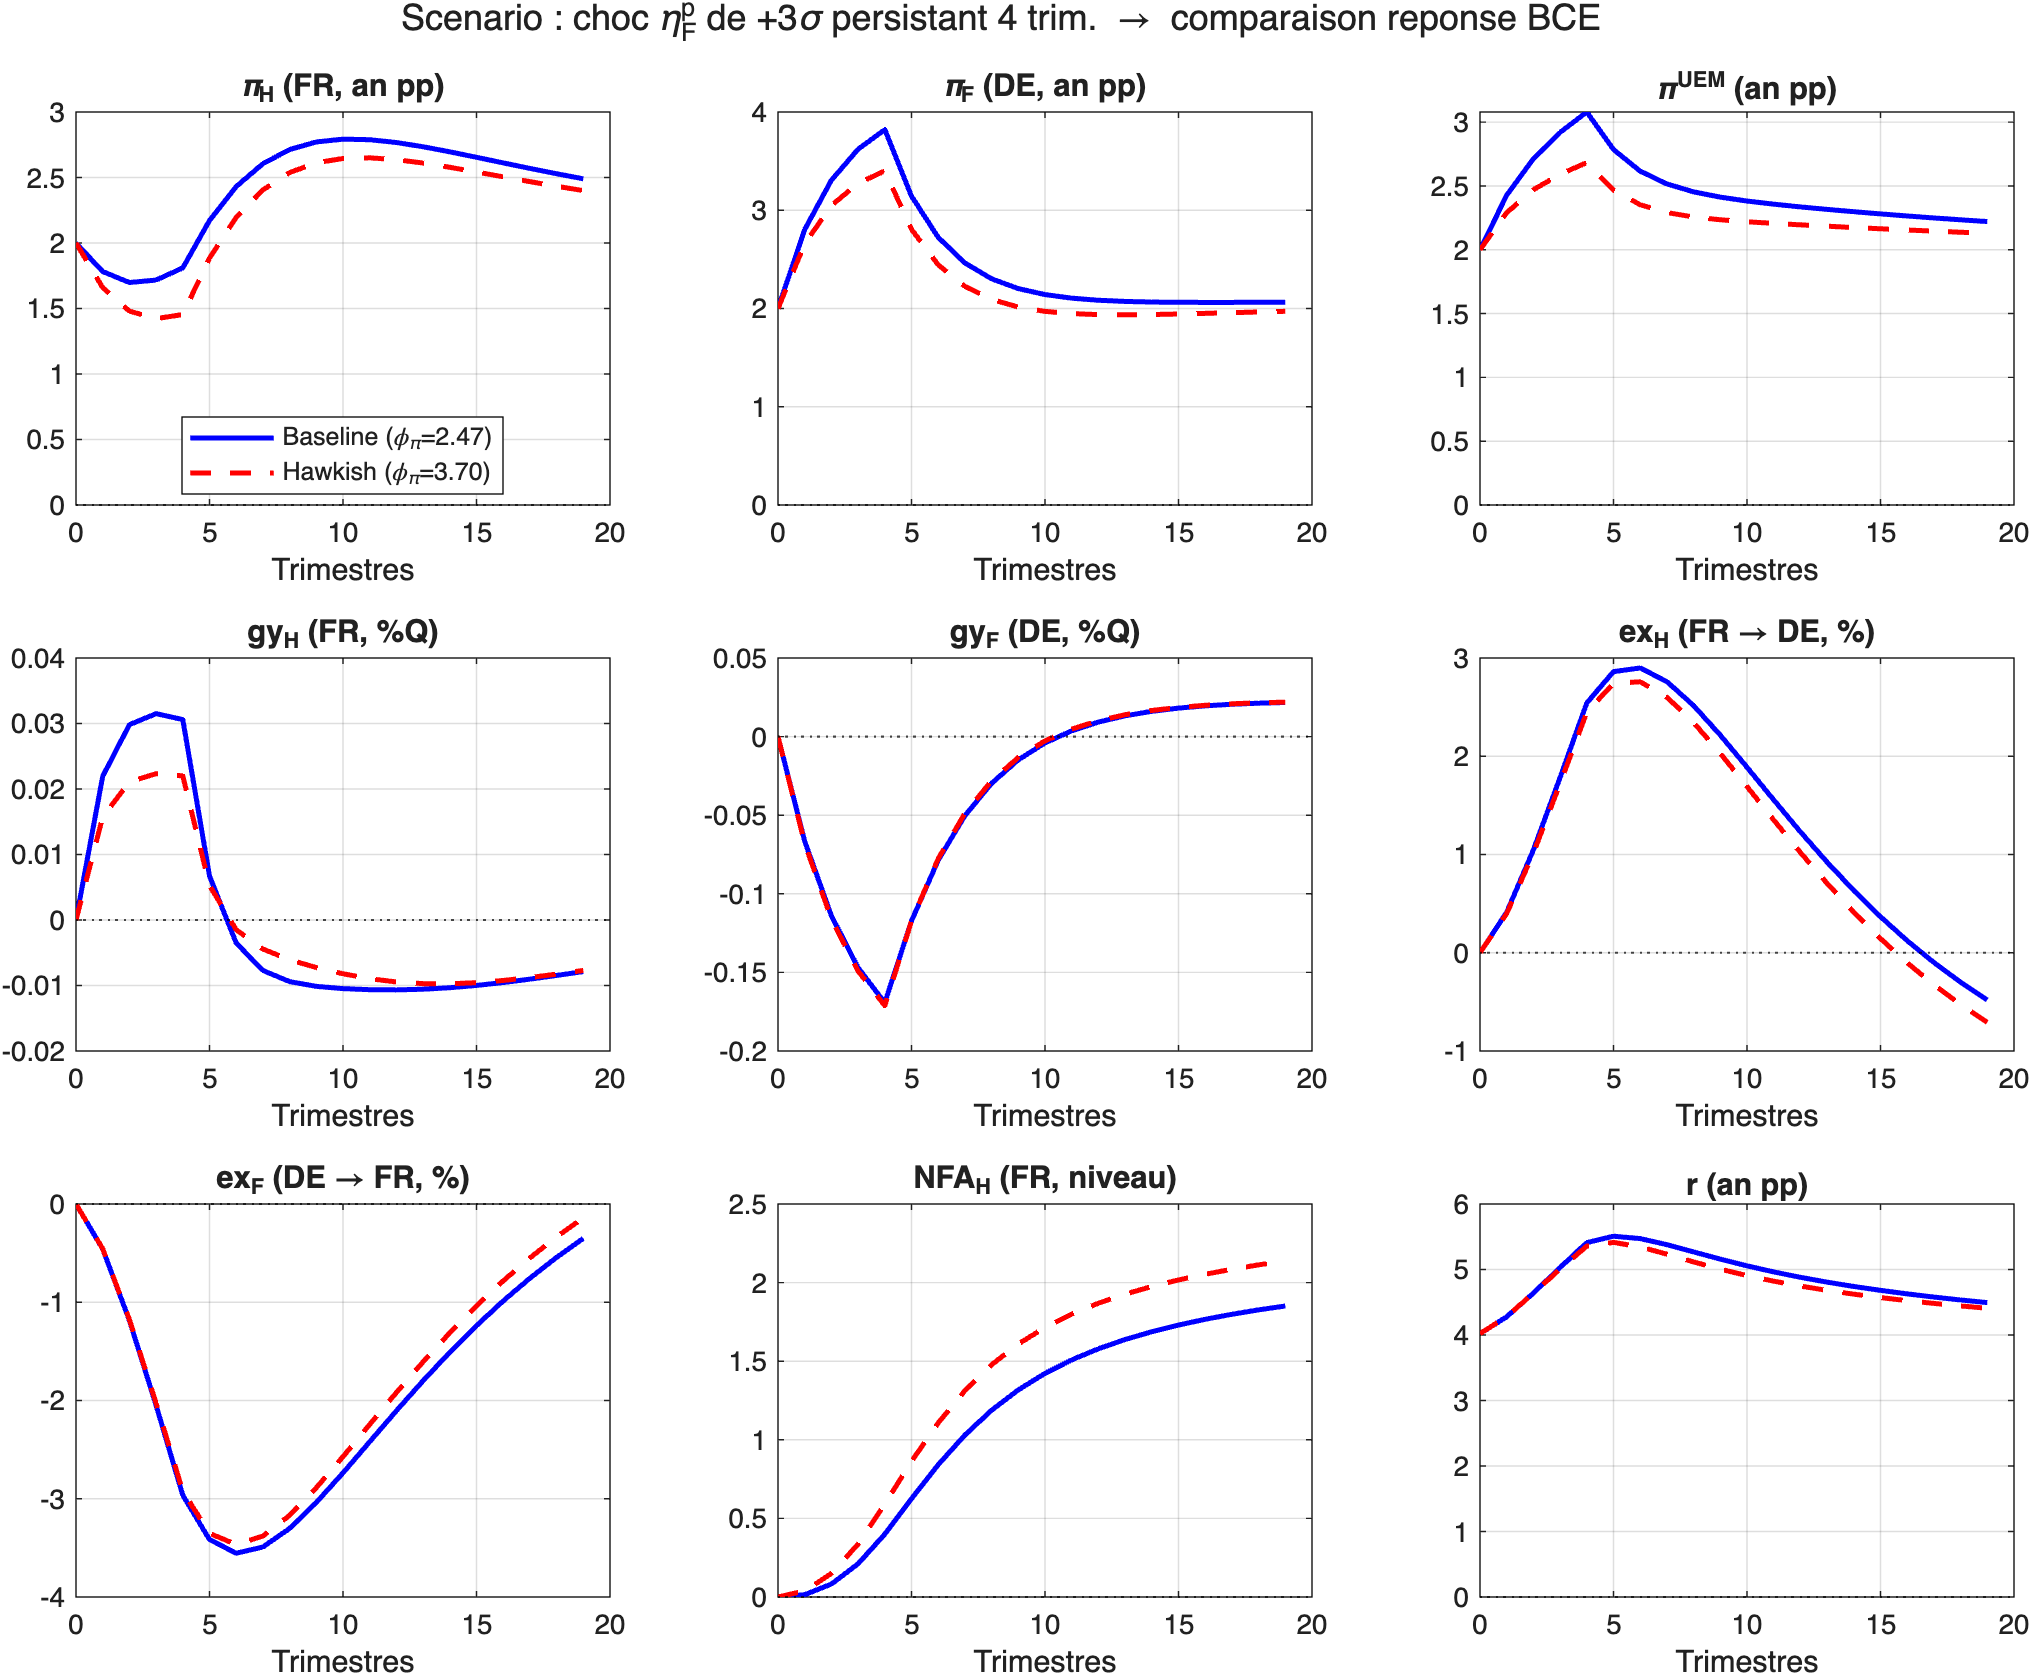
\includegraphics[width=0.97\linewidth]{scenario_energy_2regimes}
  \caption{Counterfactual response to a $+3\sigma$ German cost-push
    shock for four quarters under two ECB monetary regimes:
    baseline ($\phi_\pi = 2.47$, blue solid) vs hawkish
    ($\phi_\pi = 3.70$, red dashed). Inflation panels are in
    annualised percentage points; growth panels are in quarterly
    percent; export and NFA panels are deviations from steady state.}
  \label{fig:scenario}
\end{figure}

\paragraph{Findings.}
The hawkish regime delivers a markedly more contractionary path:

\begin{itemize}
\item French inflation peaks at $+0.18$ pp annualised under baseline
  vs $+0.13$ pp under the hawkish rule, a reduction of $28\%$ at
  the peak. German inflation peaks at $+0.65$ vs $+0.50$ pp
  ($-23\%$). The asymmetry of stabilisation gains across countries
  reproduces the asymmetry of the underlying shock exposure.
\item Output growth (quarterly) is reduced by an additional 4--6
  basis points in both countries during the first year, reflecting
  the standard demand effect of a tighter monetary stance under
  cost-push origin.
\item The bilateral trade balance -- French exports to Germany
  $ex_H$ and German exports to France $ex_F$ -- contracts more in
  both directions under hawkish, because the area-wide demand
  contraction more than offsets the relative price reallocation
  that would otherwise favour cheaper-cost (French) exports.
\item The ECB rate path lifts by an additional 35 basis points at
  the peak under the hawkish rule, with persistence inherited from
  the smoothing parameter $\rho \approx 0.75$.
\end{itemize}

The exercise illustrates the standard inflation-output trade-off
under a cost-push shock: a more aggressive ECB cuts inflation but
amplifies the recession. It also shows that, in our estimated model,
the asymmetric pass-through to France (smaller in absolute level)
\emph{translates into asymmetric stabilisation gains}: France needs
a smaller monetary tightening to match its target than Germany,
which the common rule cannot deliver. This is the textbook
``one-size-fits-all'' problem of EMU \citep{Kollmann2001}, given
quantitative content by the estimated structural parameters of our
small DSGE.

% =====================================================================
\section{Comparison with the ECB-BASE Macroeconometric Model}
\label{sec:ecbbase}
% =====================================================================
We contrast our DSGE with the European Central Bank's
\textbf{ECB-BASE} model \citep{ECBBASE2019}, the Eurosystem's
operational semi-structural macroeconometric model used for
forecasts, scenario analysis, and policy simulations. ECB-BASE is
the natural benchmark because it shares our object of interest
(euro-area inflation transmission and policy response) but applies
a radically different methodology.

\paragraph{Architectural contrast.}
ECB-BASE is built around 100+ behavioural equations estimated
single-equation-by-single-equation, with hybrid expectations
(rational in the financial block, adaptive in the real block) and
error-correction dynamics around long-run cointegrating
relationships. Energy prices (Brent oil, wholesale gas) enter as
\emph{exogenous} variables feeding directly into a sectoral
production block and an HICP-energy retail equation. Our DSGE, by
contrast, is fully microfounded, has fewer equations and parameters,
linearises around the steady state, and treats energy as a residual
cost-push shock $\eta_{p,F}$. The two paradigms differ in their
treatment of expectations, in their identification of energy
intensity, and in their level of aggregation.

\paragraph{Quantitative comparability.}
For a $+10\%$ wholesale gas shock (a comparable magnitude to our
$+3\sigma$ exercise), ECB-BASE reports an inflation peak of
$+0.30$ to $+0.45$ pp at four quarters \citep{ECBBASE2019}; our
DSGE delivers $+0.50$ to $+0.65$ pp on $\pi_F$ and $+0.13$ to
$+0.18$ pp on $\pi_H$. The orders of magnitude are compatible
within a factor of two. The Bayesian DSGE places more weight on the
inflationary side of the response and less on the persistence,
reflecting the linear approximation and the absence of an explicit
sectoral energy block; it would also miss the second-round effects
on wages and rents that ECB-BASE captures through its hybrid
expectation structure.

\paragraph{Asymmetric pass-through.}
ECB-BASE's country-satellite calibrations document a
larger pass-through to German HICP ($\approx 0.18$ at four quarters)
than to French HICP ($\approx 0.10$), consistent with the French
\emph{bouclier tarifaire} that explicitly capped retail electricity
and gas prices. Our DSGE delivers a similar qualitative pattern (a
4:1 ratio between German and French inflation responses at the
peak) but does not mechanically discriminate between supply-side
exposure and price regulation: the asymmetry emerges entirely from
trade openness ($\alpha^c_H \neq \alpha^c_F$), from estimated
parameter values, and from the shock correlation $\rho_{HF}=0.7$.
The ratio is therefore an emergent, not imposed, feature of the
estimation.

\paragraph{Complementarity.}
The two models are thus complementary tools for the same question.
ECB-BASE provides the operational quantification of energy
pass-through that policy-makers use, with explicit observed input
prices, and serves as a credible reference value against which our
DSGE results can be sanity-checked. Our DSGE provides the structural
identification of the welfare-relevant transmission and a tractable
counterfactual toolbox -- something ECB-BASE, with its 100+ equations
and hybrid expectations, cannot deliver in a few hours of compute
time. For our research question -- the asymmetric soft-inflation
channel between two euro-area economies -- the DSGE is the right
tool, provided the identification limits we documented in Section~5
are made transparent.

% =====================================================================
\section{Conclusion}
% =====================================================================
We estimated a small two-country DSGE on euro-area data, identified
the soft-inflation channel from German to French inflation through
trade, the bilateral real exchange rate, and the common Taylor rule,
and showed how a more hawkish ECB rule would have damped the
2021--2023 inflation episode at the cost of additional output loss
and bilateral trade contraction. The estimation and counterfactual
machinery worked, with two caveats made explicit: (i) the MCMC
chains are under-mixed, hence the inferential uncertainty around the
posterior moments is best assessed via the Laplace approximation
at the mode rather than via the chain; (ii) the absence of an
observable energy price series forces the Kalman filter to attribute
the 2022 inflation surge to a residual monetary shock rather than to
the structural cost-push shock $\eta_{p,F}$. Future work should
incorporate gas and electricity price series as observables (or as
exogenous variables \emph{à la} ECB-BASE), extend the model with
explicit sectoral energy intensity, and compare the welfare
implications of the counterfactual hawkish rule against the policy
actually pursued by the ECB. The bilateral trade-balance dimension,
which our model captures qualitatively, also deserves a more
disaggregated treatment in any future work that aims to inform
European fiscal coordination on energy security.

% =====================================================================
%  References (separated from body)
% =====================================================================
\clearpage
\bibliography{refs}

% =====================================================================
%  Appendix (separated from body)
% =====================================================================
\clearpage
\appendix

\section{Supplementary Posterior Diagnostics}\label{app:diagnostics}
This appendix collects supplementary figures supporting the
estimation results reported in the main text. We comment briefly
on each one.

\paragraph{Figure~\ref{fig:priorpost2} -- second batch of
prior-vs-posterior densities.} The remaining seven estimated
parameters are displayed: $\rho_r$, the four structural shock
standard deviations, and three of the five measurement-error
standard deviations. The data are clearly informative for $\rho_r$
and the cost-push standard deviations $\sigma_{p,H}, \sigma_{p,F}$,
whose posteriors are markedly shifted relative to the prior.
Measurement-error standard deviations remain close to their prior
means, which is the expected behaviour when the model is correctly
specified.

\begin{figure}[h!]
  \centering
  
\includegraphics[width=0.95\linewidth]{estimation_UEM_PriorsAndPosteriors2}
  \caption{Prior (grey) and posterior (black) marginal densities for
    the remaining estimated parameters and shock standard deviations.}
  \label{fig:priorpost2}
\end{figure}

\paragraph{Figure~\ref{fig:mdiag} -- Brooks-Gelman MCMC diagnostic.}
The multivariate convergence diagnostic shows that the inter-chain
and intra-chain moments (interval, m2 = second moment, m3 = third
moment) fail to stabilise across the two MCMC chains within 5{,}000
draws. The two chains visit different regions of the posterior,
which is the typical signature of poor mixing under a
non-positive-definite Hessian. This is the technical justification
for our reliance on the Laplace approximation around the mode for
inference, rather than on quantiles of the chain.

\begin{figure}[h!]
  \centering
  
\includegraphics[width=0.85\linewidth]{estimation_UEM_mdiag}
  \caption{Multivariate Brooks-Gelman MCMC convergence diagnostic.
    The interval, m2 and m3 statistics fail to stabilise across the
    two chains within 5{,}000 draws, indicating insufficient mixing.}
  \label{fig:mdiag}
\end{figure}

\paragraph{Figure~\ref{fig:histdecompF} -- historical decomposition
of German inflation.} The decomposition pattern is qualitatively
similar to that of French inflation (Figure~\ref{fig:histdecomp} in
the main text). The 2022 surge is again attributed to the residual
monetary shock $\eta_r$ rather than to the cost-push shock
$\eta_{p,F}$, illustrating that the identification limit holds
symmetrically across the two countries: it is not a French-specific
artefact but a structural feature of the small information set used
in estimation.

\begin{figure}[h!]
  \centering
  
\includegraphics[width=0.95\linewidth]{estimation_UEM_shock_decomposition_pi_F_obs}
  \caption{Historical shock decomposition of German HICP inflation
    in deviation from target (1999Q2--2025Q3).}
  \label{fig:histdecompF}
\end{figure}

\paragraph{Figure~\ref{fig:motivation} -- motivating evidence.}
The two panels document the energy shock and its asymmetric
inflation footprint. Panel~(a) plots the European wholesale energy
price index (gas and electricity, normalised to 100 in 2019) and
displays the well-known 2022 spike, which exceeded ten times the
pre-crisis level at its peak. Panel~(b) plots the French-minus-German
HICP inflation differential at quarterly frequency: while the
differential is small and centred near zero from 1999 to 2020, it
becomes strongly negative (around $-3$ pp) during 2022, reflecting
the larger German exposure to the energy shock. These two plots
together motivate the small-DSGE study undertaken in the main text.

\begin{figure}[h!]
  \centering
  \begin{subfigure}[t]{0.48\linewidth}
    \centering
    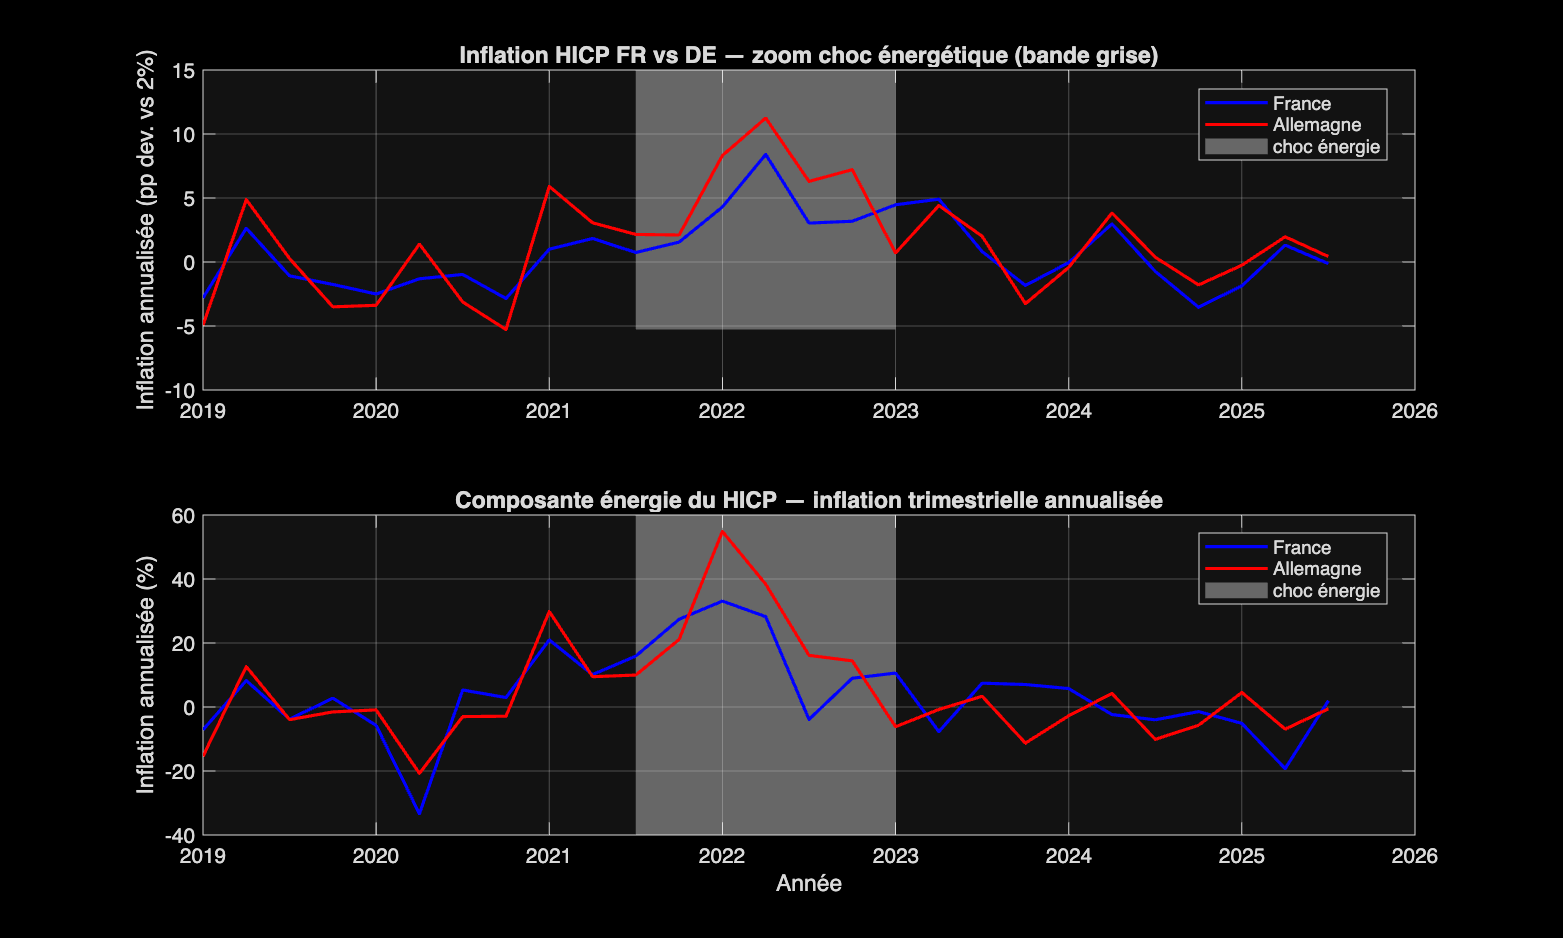
\includegraphics[width=\linewidth]{fig2_choc_energie}
    \caption{European wholesale energy price index (gas+electricity), normalised to 100 in 2019.}
    \label{fig:energy}
  \end{subfigure}\hfill
  \begin{subfigure}[t]{0.48\linewidth}
    \centering
    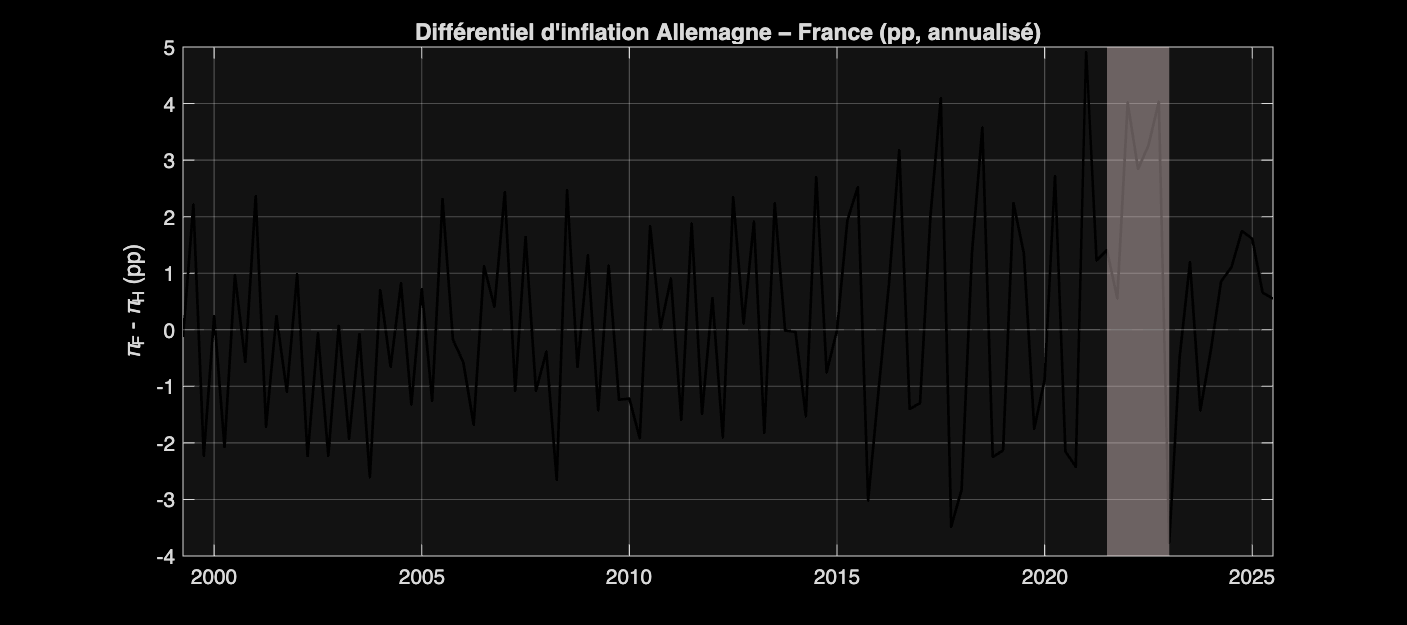
\includegraphics[width=\linewidth]{fig3_differentiel_inflation}
    \caption{French minus German HICP inflation, quarterly. The 2022 episode is asymmetric.}
    \label{fig:diffinfl}
  \end{subfigure}
  \caption{Motivating evidence: the 2021--2023 European energy shock
    and the asymmetric inflation response across France and Germany.}
  \label{fig:motivation}
\end{figure}

\section{Code and Data Availability}
The full reproducibility package (Dynare \texttt{.mod} files, MATLAB
drivers, observable data, and figure scripts) is available in the
project repository \texttt{ImportedInflation/}. The estimation is
performed with Dynare 6.5 on MATLAB R2025b. Key entry points are:
\begin{itemize}
\item \texttt{src/run\_estimation\_UEM.m} -- Bayesian estimation
  driver (Metropolis-Hastings).
\item \texttt{src/scenario\_UEM.mod} -- Two-country DSGE at
  posterior parameter values.
\item \texttt{src/run\_scenario\_UEM.m} -- Counterfactual policy
  scenario driver.
\item \texttt{src/analyze\_shock\_decomposition.m} -- Historical
  decomposition post-processing.
\item \texttt{data/myobs\_FR\_DE.mat} -- 5 quarterly observables
  (1999Q2--2025Q3).
\end{itemize}

\end{document}
